\chapter{Analyzing vocabulary} \label{ch:vocabulary}

\epigraph{Language is unfinished business. Words come, words go, taking their chances like everyone else.}{}

\section{Introduction} \label{sec:intro}

For many people, language is all about words. It's not that they discount grammar, but words are just so salient, and there are so very many of them. Grammar provides the architecture; vocabulary furnishes the rooms.

This chapter examines vocabulary as a linguistic phenomenon:

\begin{itemize}[noitemsep]
\item How words are constructed (morphology)
\item What constitutes a ``word'' and different ways to count vocabulary
\item The frequency distribution of words in English
\item How vocabulary size relates to text coverage
\item The relationship between vocabulary and other aspects of language
\item Common misconceptions that can derail vocabulary instruction
\end{itemize}

We begin by examining the building blocks of vocabulary: morphemes and word formation. This foundation will inform our subsequent discussions on vocabulary size, frequency, and the various ways linguists conceptualize and count words.

\section{What's a word}\label{sec:what-is-a-word}

Defining exactly what constitutes a ``word'' is trickier than it might seem at first glance. The complexity arises from multiple perspectives on what counts as a word and how words relate to each other through morphological processes.

In this section, we'll consider:

\begin{itemize}[noitemsep]
   \item Semantic vs syntactic notions of a word
   \item How words are formed and change (morphology)
   \item Different ways of conceptualizing words for various purposes
   \item The relationship between word forms and word families
\end{itemize}

\subsection{Semantic and syntactic notions of words}

When discussing words, it's useful to distinguish between the semantic and syntactic perspectives. They don't always coincide, and sometimes misunderstandings are simply due to a lack of a shared perspective.

From a semantic standpoint, a word is a unit of meaning. This view focuses on the conceptual content rather than grammatical behaviour. Dictionaries typically reflect this perspective, treating semantically unified strings such as \href{https://www.ldoceonline.com/dictionary/at-the-moment}{\textit{at the moment}}, meaning `now' as single entries even when they consist of multiple syntactic parts. A prime example of this is the treatment of so-called ``phrasal verbs'' (See \ref{ssec:phrasal-verbs}).\footnote{Phrasal verbs like \textit{put up with} are often only phrases in the traditional sense of `a group of words' and not in the technical sense of a `a syntactic head and its dependents'.} Consider the case of \textit{give up}:

\ea \textit{I decided to \uline{give up} smoking.}
\z

\noindent Semantically and lexicographically, \textit{give up} functions as a single unit of meaning `stop doing or trying something'. You'd find it as one entry in a dictionary, despite its two-part composition.

Syntactically, though, we often need to treat the components of such expressions as separate words. This is the view we've been employing in our discussions of lexical categories in earlier chapters. From this angle, \textit{give} and \textit{up} are distinct syntactic units, a verb and a preposition, as evidenced by their ability to be separated in certain constructions:

\ea
\ea \textit{I \uline{gave up} smoking last year.}
\ex \textit{I \uline{gave} it \uline{up} last year.}
\z\z

This syntactic flexibility demonstrates why, grammatically, we often need to consider \textit{give} and \textit{up} as separate words, even when it takes both to convey the intended meaning.

Both perspectives are valid: semantics asks what words mean, syntax asks how meanings work as words. Pay attention to which perspective is in play.

While these different notions of words help us understand their behaviour in phrases and sentences, there's another crucial aspect to consider: how words themselves are formed and how they change. This brings us to the study of morphology.

\subsection{Morphology} \label{sec:morphology}

\textsc{Morphology} is the study of how words change their form or category, how they morph. For example, the fact that you can add \textit{-ly} to the adjective \textit{happy} and get the adverb \textit{happily} is a morphological fact. As is the fact that you can get the noun \textit{run} from the verb \textit{run} without changing anything at all. Some languages are rich in morphology, but English is relatively impoverished in this regard.

Words can be formed of \textsc{bases} and \textsc{affixes}\is{affix, affixation}. All words contain at least one base\is{base (morphological)}, and most bases are words in their own right. For example, the base of \textit{happiness} is \textit{happy}, which is obviously a word. In contrast, \textit{-ness} is an affix, which depends on a base. This is very much like the syntactic idea of heads (Section \ref{sec:head}) and dependents (Section \ref{sec:Dep}). But just as some syntactic heads, such as the verb \textit{helped}, can't form a sentence on their own, some bases cannot stand alone as words. One example is \textit{dur}, as in \textit{durable} or \textit{duration}. \textit{Dur} is never a word on its own, but nor does it combine with any free bases.

There are also special bases called \textsc{combining forms}\is{combining form}. These include examples such as \textit{bio} and \textit{ology}, which combine to form words such as \textit{biology}. Combining forms usually combine with each other, but sometimes they can combine with a free base, as in \textit{bio-mechanical}. The distinction between combining forms and affixes isn't always clear-cut. Elements like \textit{tele-} (as in \textit{television}) or \textit{mini-} (as in \textit{miniskirt}) started as combining forms but now function more like prefixes. The key difference is that true combining forms typically derive from Greek\il{Greek} or Latin\il{Latin} roots and often combine with other bound forms, while affixes attach to existing words.\footnote{For a detailed discussion of the combining form/affix boundary, see \citet{Bauer1983}.}

\subsection{Derivation and inflection} \label{sec:derivation}\is{derivation, derivative|(}\is{inflection|(}

English employs two types of morphological processes: derivation and inflection. \textsc{Derivational morphology} creates new words or changes a word's lexical category. \textsc{Inflectional morphology} marks grammatical distinctions without creating new words.

\subsubsection*{Derivational affixes}

According to \textit{The Longman grammar of spoken and written English} \citep[401]{Biber1999}, certain affixes stand head and shoulders above others in terms of their frequency in a 40-million-word corpus.

\paragraph*{Verb-forming suffixes} These suffixes change words into verbs. For example, to describe somebody's character is to \textit{characterize} them. The verb \textit{characterize} is formed by adding the verb-forming suffix \textit{-ize} to the noun \textit{character}. The most common verb-forming suffixes, occurring in roughly 20--170 verbs each, are: \textit{-ize}/\textit{-ise}, \textit{-en}, \textit{-ate}, and \textit{-}(\textit{i})\textit{fy}.

\paragraph*{Verb-changing prefixes} These prefixes change the meaning of the verb without changing its lexical category. For example, if you \textit{overdo} something, you do it too much. But both \textit{do} and \textit{overdo} are verbs. The most common of these prefixes are: \textit{re-}, \textit{over-}, \textit{un-}, \textit{mis-}, and \textit{out-} \citep[400]{Biber1999}.

\paragraph*{Noun-forming suffixes} These suffixes change adjectives and verbs into nouns. For example, \textit{openness} is the adjective \textit{open} + the suffix \textit{-ness}. The most productive are: \textit{-tion}, \textit{-ism}, \textit{-ity}, \textit{-ness}, \textit{-ment}, \textit{-ant}, \textit{-ship}, \textit{-age}, and \textit{-ery}.

There are about 2,000 nouns ending in \textit{-tion} in the Longman grammar's corpus, and only about 50 ending in \textit{-ery}. This dramatic difference in frequency between the most frequent and even slightly less frequent elements is a fundamental pattern we'll see repeated across various aspects of vocabulary (e.g., in Section \ref{sec:word-frequency}).\is{derivation, derivative|)}

\subsubsection*{Inflectional suffixes}

English has a limited set of inflectional suffixes that mark grammatical systems: tense, number, and comparison. These include: the possessive \textit{'s}, the verbal suffixes \textit{-s}, \textit{-ed}, and \textit{-ing} (see Section \ref{sec:verb-forms}), the plural \textit{-s} on nouns, and the comparative \textit{-er} and superlative \textit{-est} on adjectives and adverbs. Unlike derivational morphology, inflectional morphology doesn't create new words or lexical categories.

\begin{tcolorbox}[title=Exercise: Understanding Word Structure, colback=white, colframe=blue!75!black, fonttitle=\bfseries]
1. The words \textit{biology}, \textit{biography}, and \textit{biodegradable} all begin with \textit{bio-}. 
 \begin{enumerate}[nosep]
 \item What does this element mean, and why might it combine with both Greek\il{Greek}-origin elements (like \textit{-logy}) and English words (like \textit{degradable})?
 \item How does this differ from a prefix like \textit{un-}, which attaches to existing English words?
 \end{enumerate}

2. Consider the verb \textit{sing}: \textit{sing}, \textit{sings}, \textit{singing}, \textit{sang}, \textit{sung}.
 \begin{enumerate}[nosep]
 \item Why do dictionaries list all these forms under one entry?
 \item How does this help explain why English dictionaries have fewer entries than the total number of word forms in English?
 \end{enumerate}

3. A student writes: ``I looked it up in the dictionary but couldn't find \textit{happily}.'' 
 What linguistic knowledge would help them find this word, and what does this tell us about how dictionaries organize information?
\end{tcolorbox}

\subsection{Word families, lemmas, shapes, and tokens}\label{sec:family-lemma-shape-token}\is{derivation, derivative|(}

The variability of word forms through inflection and derivation makes counting words surprisingly complex. How do we account for words like \textit{wide}, \textit{wider}, and \textit{width}? Are they separate words, or just variations of the same word? Linguists use several different ways of grouping and counting words, each serving different purposes. See Figure \ref{fig:wide-family-tree}.

\paragraph*{Word families} A \textsc{word family} includes a base word and all its inflectionally and derivationally related words. All the words in the following list belong to a single word family, the \textit{wide} family: \textit{wide}, \textit{wider}, \textit{widest}, \textit{widely}, \textit{widen}, \textit{widens}, \textit{widened}, \textit{widening}, \textit{wideness}, \textit{widener}, \textit{wideners}, and \textit{width}.\footnote{You could add \textit{widespread}, \textit{wide-ranging}, \textit{wide-eyed}, etc.}

The size and composition of word families isn't fixed but relates to morphological transparency. A word family includes a base word plus its inflected and derived forms, but which derived forms belong to a family depends on how transparent the morphological relationship is. For instance, \textit{industry} and \textit{industrious} clearly belong to the same family, while etymologically\is{etymology} related pairs like \textit{abyss}/\textit{abysmal} may not be recognized as related by most speakers.

\paragraph*{Lemmas} The inflectionally related words belong to a single \textsc{lemma}. For example, the verb lemma \textit{widen} includes \textit{widen}, \textit{widens}, \textit{widened} (past tense), \textit{widened} (past participle), and \textit{widening}. The \textit{wide} family includes several lemmas: an adjective \textit{wide}, an adverb \textit{widely}, a verb \textit{widen}, and two nouns \textit{widener} and \textit{width}. Generally, a lemma is what you look up in the dictionary.

\paragraph*{Word shapes} Each inflectional or derivational word form is a different \textsc{shape} (\textit{type} is another commonly used term).\footnote{The term \textsc{shape} is often preferred by syntacticians; \textsc{type} is more common in philosophy.} In the \textit{wide} lemma, there are three shapes: \textit{wide}, \textit{wider}, and \textit{widest}.\is{inflection|)}\is{derivation, derivative|)}

\paragraph*{Word tokens} A \textsc{word token} is a single instance or occurrence of a word in a text or utterance. If an article is 800 words long, it has 800 tokens, even if 56 of those tokens are \textit{the}.

\begin{figure}[htbp]
\centering
\begin{forest}
for tree={
 grow=east,           % Tree grows downwards
 l sep=8mm,            % Reduced vertical spacing between levels
 s sep=5mm,            % Reduced horizontal spacing between siblings
 anchor=center,
 edge={-stealth},
 inner sep=1pt,        % Minimal padding around text
}
[\texttt{family}\\wide, align=center
 [\texttt{lemma}\\wide (adj), align=center
   [\texttt{shape}\\wide, align=center
     [\texttt{token}\\\textit{a \uline{wide} river}, align=center]
   ]
   [\texttt{shape}\\wider, align=center
     [\texttt{token}\\\textit{a \uline{wider} river}, align=center]
   ]
   [\texttt{shape}\\widest, align=center
     [\texttt{token}\\\textit{the \uline{widest} river}, align=center]
   ]
 ]
 [\texttt{lemma}\\widen (verb), align=center
   [\texttt{shape}\\widen, align=center
     [\texttt{token}\\\textit{to \uline{widen} the gap}, align=center]
   ]
   [\texttt{shape}\\widens, align=center
     [\texttt{token}\\\textit{the gap \uline{widens}}, align=center]
   ]
   [\texttt{shape}\\widened, align=center
     [\texttt{token}\\\textit{they \uline{widened} it}, align=center]
   ]
 ]
 [\texttt{lemma}\\width (noun), align=center
   [\texttt{shape}\\width, align=center
     [\texttt{token}\\\textit{the \uline{width} of}, align=center]
   ]
 ]
]
\end{forest}
\caption{A tree diagram illustrating the relationship between a word family, its lemmas (with part-of-speech), types (inflected forms), and contextual tokens. The diagram uses the \textit{wide} family as an example.}
\label{fig:wide-family-tree}
\end{figure}

These different conceptualizations of words serve different purposes. Dictionaries typically count lemmas. Researchers studying a person's vocabulary size often work with word families. Text length is measured in tokens. Interpreting linguistic data and research correctly requires an understanding of these distinctions.

\begin{tcolorbox}[title=Exercise: Word Families and Lemmas, colback=white, colframe=blue!75!black, fonttitle=\bfseries]
1. For each of the following, list at least three other words that belong to the same word family:

\begin{enumerate}[nosep]
   \item \textit{happy}
   \item \textit{create}
   \item \textit{science}
   \item \textit{electric}
   \item \textit{politics}
\end{enumerate}
\medskip
2. Identify the lemma(s) for each of the following words:

\begin{enumerate}[nosep]
   \item \textit{running}
   \item \textit{better}
   \item \textit{mice}
   \item \textit{went}
   \item \textit{lives}
\end{enumerate}
\medskip
3. Explain the difference between a word family and a lemma, using examples from your answers above.
\end{tcolorbox}

\section{Word frequency and distribution} \label{sec:word-frequency}

Having established how words can be analyzed and counted, we can now examine how these different word forms are distributed in actual use. Word frequency plays a fundamental role in understanding how vocabulary functions in English. Corpus linguistics research demonstrates that a relatively small number of high-frequency words account for a large percentage of tokens in typical texts.

\subsection{The frequency distribution}

Word frequency in English (in fact in all human languages) follows a stark pattern: a few words dominate, most languish. The most frequent word (\textit{the}) occurs about 60,800 times per million words, while the 100th most frequent word (\textit{such}) occurs only about 900 times per million. By the time we reach the 1,000th most frequent word (\textit{purchase}), frequency has dropped to about 90 occurrences per million words. This pattern~-- where a few items account for most occurrences~-- is known as a Zipfian distribution, and it has implications for vocabulary coverage and comprehension.

\begin{table}[ht]
\centering
\caption{Word frequency drop-off}
\label{tab:word-frequency}
\begin{tabular}{lrr}
\toprule
\textbf{Word family} & \textbf{Rank} & \textbf{Frequency per million words} \\
\midrule
\textit{the} & 1 & 60,800 \\
\textit{you} & 10 & 12,800 \\
\textit{such} & 100 & 900 \\
\textit{purchase} & 1,000 & 90 \\
\textit{negotiate} & 2,000 & 35 \\
\bottomrule
\end{tabular}
\end{table}
These frequencies are based on the Corpus of Contemporary American English (COCA)\is{corpus!COCA}, using word family counts following \citet{nation2013}. Different corpora and counting methods will yield somewhat different figures, but the general pattern of dramatic frequency drop-off remains consistent across sources.

\subsection{Vocabulary size and text coverage} \label{sec:vocab-size-coverage}

Very roughly, beginning learners typically know fewer than 1,000 word families, which provides basic communication ability but requires extensive circumlocution.\footnote{See Appendix \ref{ch:proficiency} for a discussion of proficiency levels.} Intermediate learners (B1--B2 in the Common European Framework) typically know up to 5,000 families, enabling participation in everyday conversations and comprehension of simplified texts. Advanced learners may know up to 8,000 families, approaching the threshold for comfortable comprehension of unsimplified texts. Proficient adult speakers of English typically know 20,000--35,000 word families, with university-educated speakers often knowing more. See Figure \ref{fig:voc-size-est}.

\begin{figure}
   \centering
   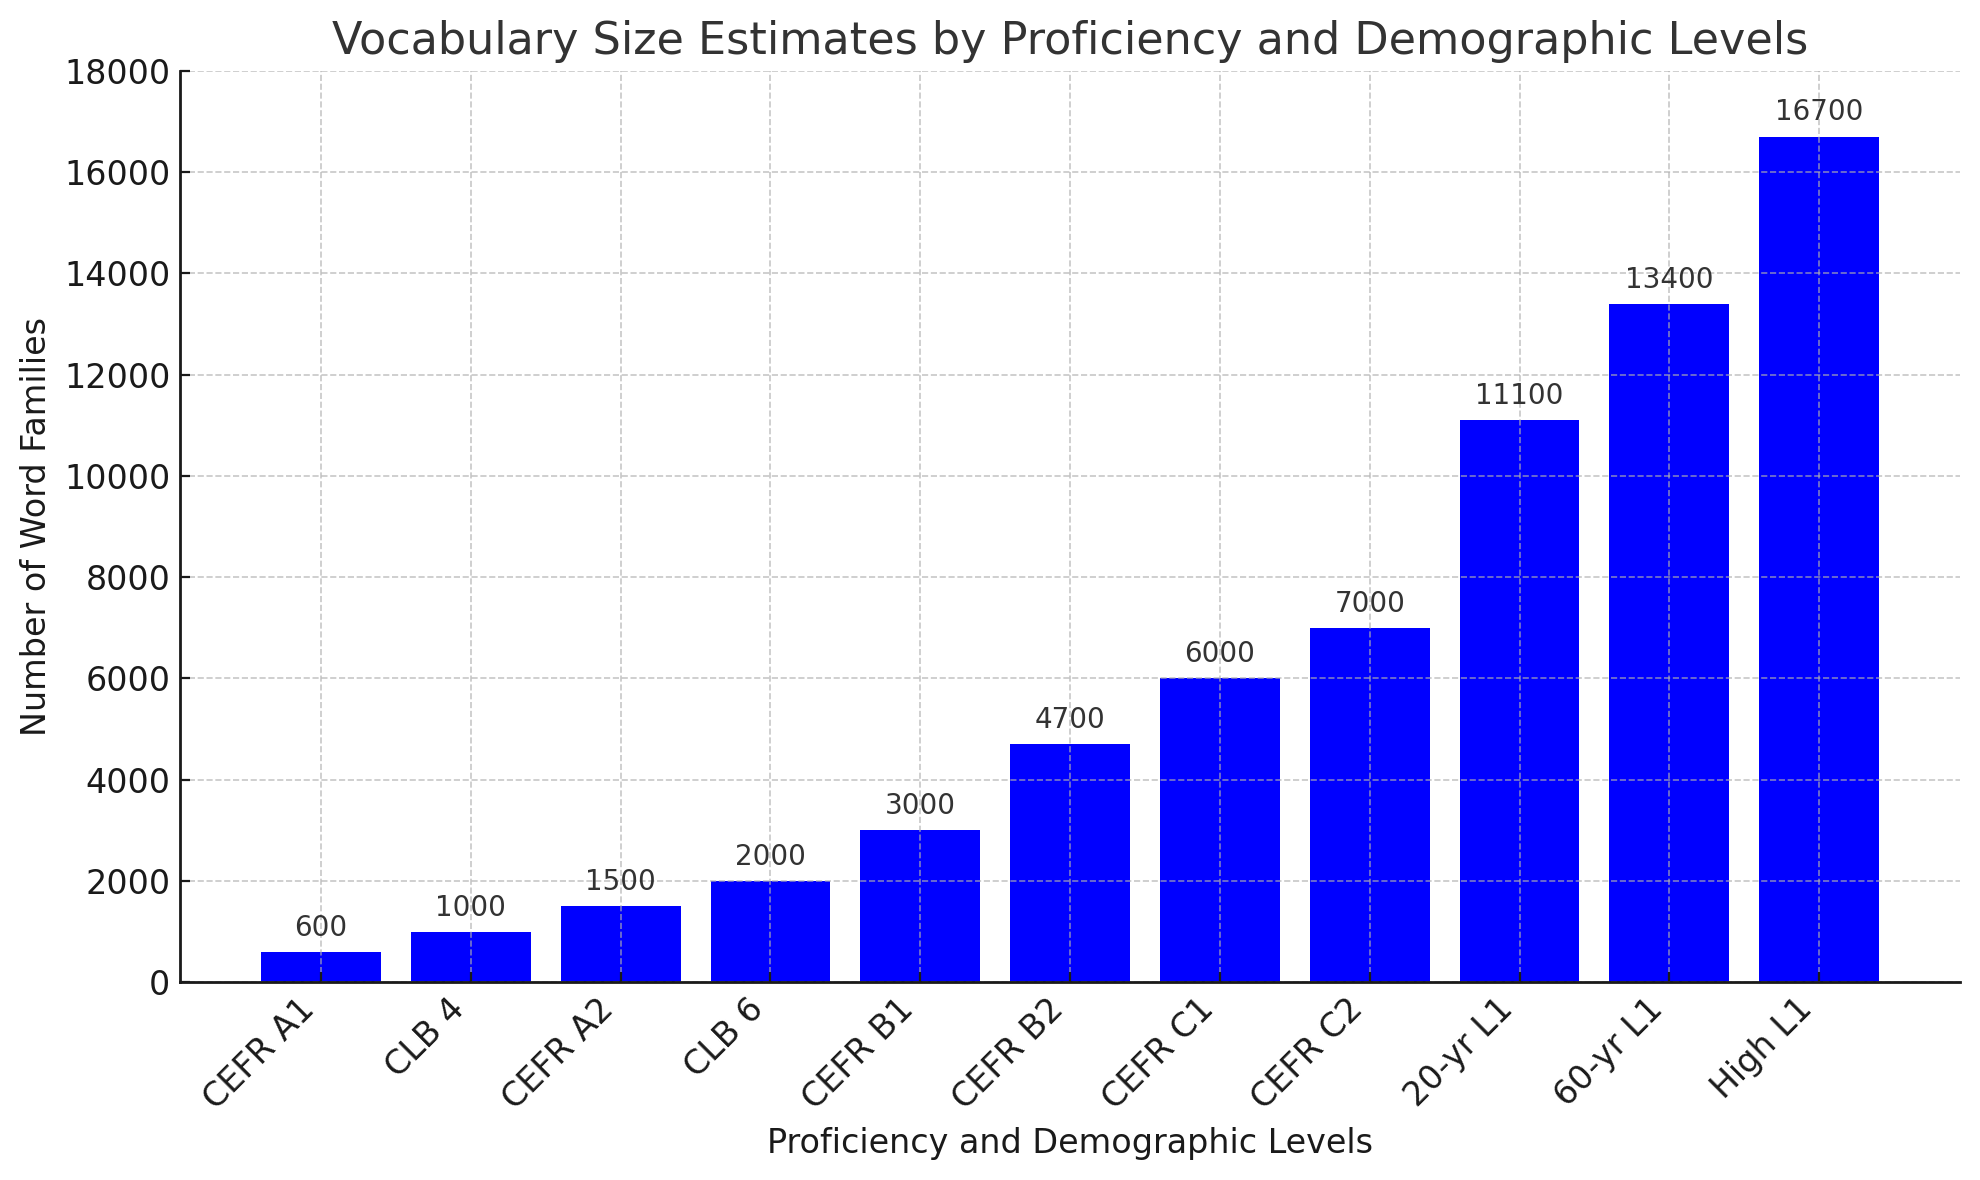
\includegraphics[width=0.8\linewidth]{figures/vocab-size-est.png}
   \caption{Vocabulary size estimates across proficiency and demographic levels based on cumulative word families \citep{brysbaert2016, capel2010, capel2012}.}
   \label{fig:voc-size-est}
\end{figure}

The relationship between vocabulary size and text coverage follows a predictable pattern shown in Figure \ref{fig:coverage-curve}. The most frequent 1,000 word families in English cover approximately 80\% of written text. The next 1,000 families add only about 6\% more coverage, and the curve continues to flatten.

\begin{figure}
\centering
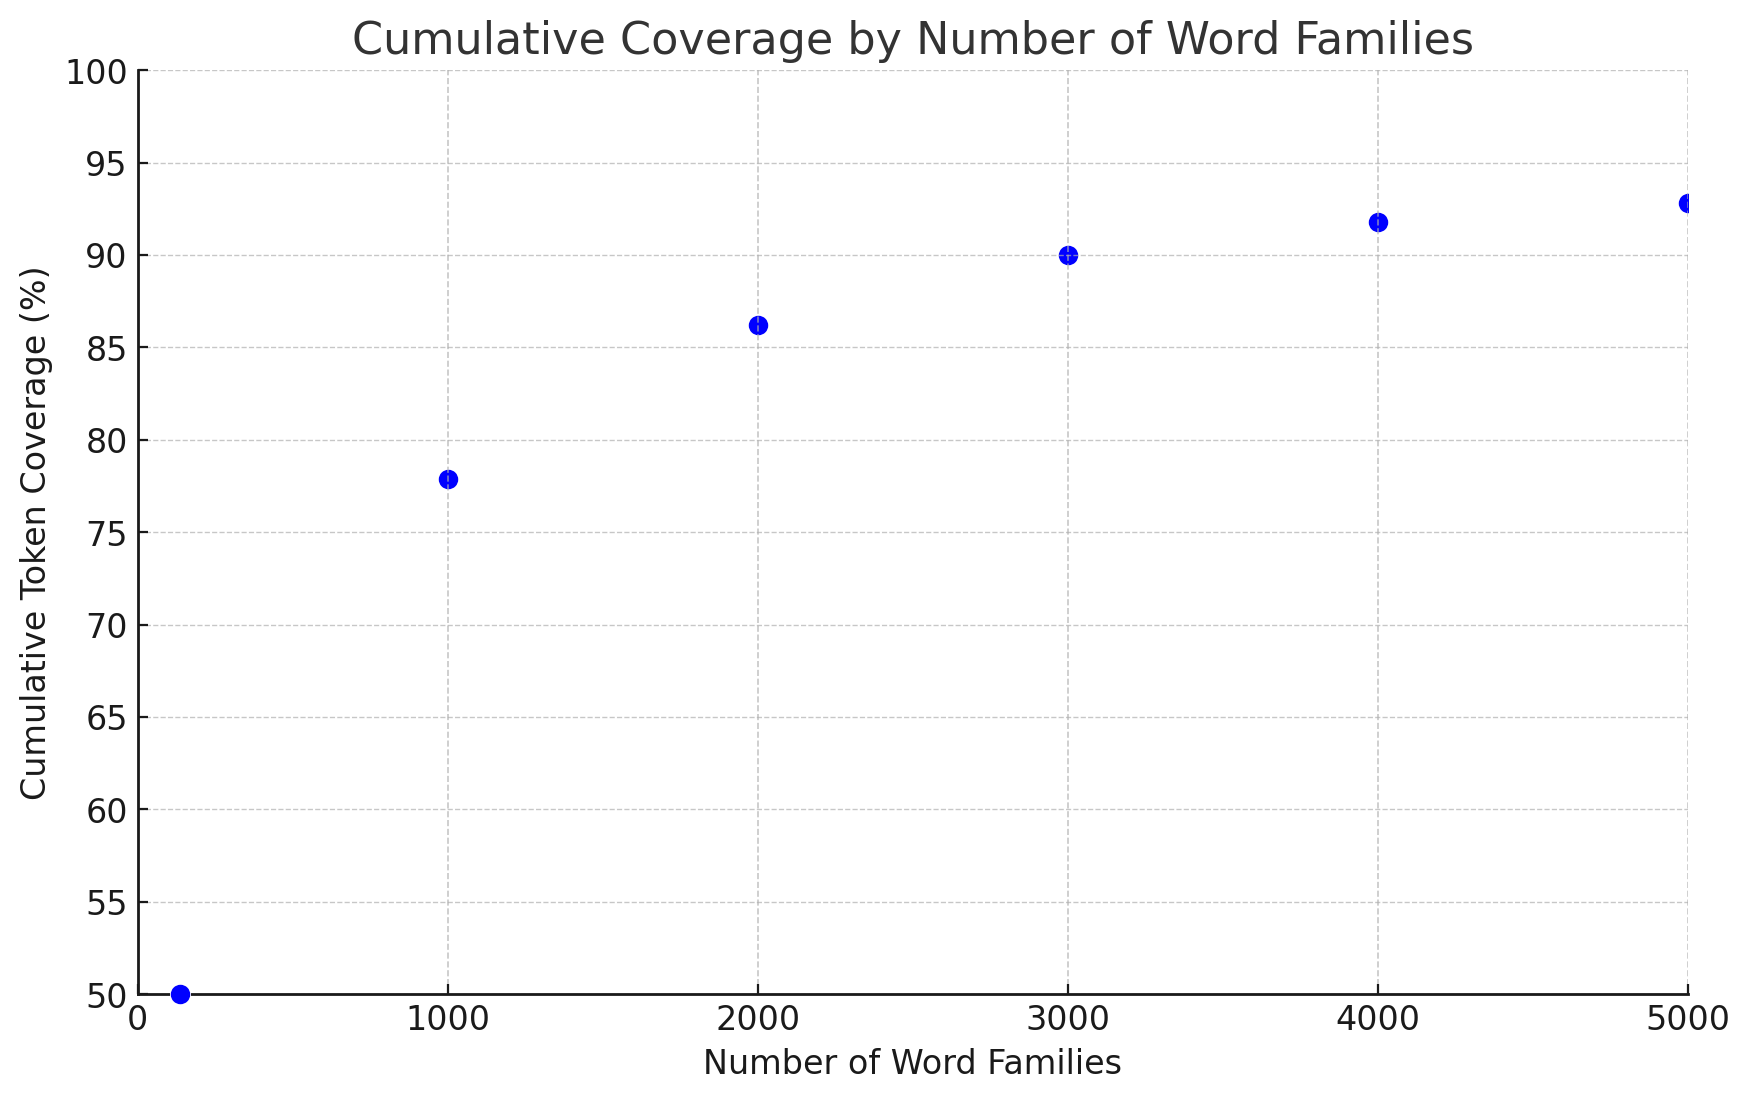
\includegraphics[width=0.8\linewidth]{figures/cumulative-families.png}
\caption{Cumulative token coverage by number of word families known}
\label{fig:coverage-curve}
\end{figure}

Research suggests that readers need to know about 98\% of the words in a text for comfortable comprehension \citep{Hu2000}. For typical reading materials like newspapers, books, and emails, this means knowing about 8,000--9,000 word families. But proper nouns (names of people, places, companies) often make up about 4\% of text \citep[29]{Nation2022}, reducing the actual vocabulary burden to about 7,800 word families.

Spoken English tends to use fewer word families than written texts. Just 2,000 families make up most words in everyday English conversation.

These figures help contextualize frequency and coverage data. When we note that the most frequent 2,000 families provide about 86\% text coverage, we can see why intermediate learners often struggle with authentic texts: knowing 86\% of words falls well short of the 98\% needed for comfortable comprehension.

\subsection{Specialized vocabulary}

Certain genres have particular sub-groups of words that occur with high frequency within those contexts. Academic English, for example, contains a core set of words that appear frequently across disciplines. The Academic Word List \citep{coxhead2000academic} identifies 570 word families that are particularly common in academic texts but less frequent in general English. Knowledge of the 2,000 most frequent general word families plus the Academic Word List provides approximately 93\% coverage of academic texts.

\begin{tcolorbox}[title=Exercise: Frequency and Comprehension, colback=white, colframe=green!75!black, fonttitle=\bfseries]
1. Here's a sentence with some words replaced by nonsense words:
 ``The scientist \textit{vexored} that the \textit{blentic} samples showed unusual \textit{tripheration} patterns.''
 \begin{enumerate}[nosep]
 \item Even without knowing the nonsense words, what can you infer about their meanings? How?
 \item What does this tell us about the relationship between high-frequency words (like \textit{the}, \textit{that}, \textit{showed}) and comprehension?
 \end{enumerate}

2. Research shows that \textit{the} appears about 60,800 times per million words, while \textit{purchase} appears three orders of magnitude less frequently.
 \begin{enumerate}[nosep]
 \item Calculate roughly how many pages you'd have to read before encountering them in a 300-page novel (assume 100,000 words).
 \item What does this dramatic difference tell us about how vocabulary is distributed in English?
 \end{enumerate}

3. An advanced learner knows 5,000 word families but struggles with newspaper articles. Using the coverage data from this chapter, explain why 5,000 families might be insufficient for comfortable reading.
\end{tcolorbox}

\section{Form, meaning, and use} \label{sec:form-meaning-use}

Understanding a word involves knowing not just its basic form and meaning but also the relational complexities among form, meaning, and use.

\subsection{Polysemy and monosemy} \label{sec:polysemy}\is{homonymy}\is{polysemy}\is{monosemy}

Most common words in English have multiple related meanings; they're \textsc{polysemous}. The word \textit{head}, for instance, can refer to the body part, the leader of an organization, the foam on beer, or the front of a line, and those are just the nouns. These meanings are related through metaphorical extension of `the top or front part of something'. (Recall the fallacy of monosomy from Section \ref{sec:fallacy-of-monosemy}.)\is{fallacy of monosemy}

Polysemy differs from \textsc{homonymy}, where unrelated words happen to share the same form. \textit{Bank} (financial institution) and \textit{bank} (river's edge) are homonyms, historically unrelated words that coincidentally have the same form.

The prevalence of polysemy in high-frequency words reflects a general pattern: common words tend to develop multiple meanings through metaphorical and metonymic extension. Less frequent words are more likely to be \textsc{monosemous}, having a single, specific meaning.

\subsection{Collocations} \label{sec:collocations}\is{collocation|(}

Words often occur in predictable combinations called \textsc{collocations}. In English, we \textit{make} a decision but \textit{take} a break (not \textit{*take a decision} or \textit{*make a break} in most varieties). We say \textit{heavy rain} (not \textit{*strong rain}) but \textit{strong wind} (not \textit{*heavy wind}). The existence of collocations reflects the partially formulaic nature of language. While syntax provides the structure for combining words, usage patterns create preferences for certain combinations over others. Corpus linguists use statistical methods to identify these patterns, finding word combinations that occur together more often than we'd expect by chance.\footnote{Common statistical measures include mutual information (MI) and t-scores, which quantify the strength of word associations.}

Collocations exist on a continuum from completely free combinations to fixed expressions. At one end, combinations like \textit{red car} are entirely compositional: any colour can modify \textit{car}. At the other end, expressions like \textit{kick the bucket} (meaning `die') are fully fixed idioms. Most collocations fall somewhere in between, showing preferences rather than absolute restrictions.\is{collocation|)}

\subsection{Idioms and formulaic language}\is{idiom|(}\is{formulaic language|(}

\textsc{Idioms} are expressions whose meaning cannot be derived from the meanings of their component words. Examples include \textit{spill the beans} (`reveal a secret'), \textit{under the weather} (`ill'), and \textit{a piece of cake} (`something easy').

Corpus studies show that individual idioms occur relatively infrequently. Even seemingly common idioms like \textit{hit the jackpot} appear rarely. This low frequency, combined with their cultural specificity and semantic opacity, makes idioms a high-investment, low-payoff aspect of vocabulary. The cultural and contextual factors that influence idiom interpretation connect to broader issues of pragmatic competence discussed in Chapter \ref{ch:pragmatics}.

Idioms represent just one type of formulaic language. Other types include:
\begin{itemize}[noitemsep]
\item Phrasal verbs (\textit{give up}, \textit{look after}), though note that not all phrasal verbs are idiomatic; some like \textit{put down} can be semantically transparent
\item Pragmatic formulas (\textit{how do you do}, \textit{nice to meet you})
\item Discourse markers (\textit{on the other hand}, \textit{as a matter of fact})
\end{itemize}

These examples highlight how much of language consists of multi-word patterns. \textsc{Construction grammar}\is{Construction Grammar} (see Section \ref{sec:constructions}) views these not as special cases but as part of how all language works: everything~-- from single morphemes to sentence patterns~-- counts as a construction, a learned pairing of form and meaning. In this view, \textit{kick the bucket}, the V + \textit{up} pattern, the word \textit{dog}, and even the plural \textit{-s} are all constructions. From this perspective, language knowledge consists of thousands of these constructions rather than words plus rules for combining them, and vocabulary isn't just individual words but all these stored form-meaning pairings, regardless of their size or complexity.\is{idiom|)}\is{formulaic language|)}

\begin{tcolorbox}[title=Exercise: Meaning and Use, colback=white, colframe=purple!75!black, fonttitle=\bfseries]
1. The lemma \textit{head} (noun) can refer to: the body part, the leader of an organization, the foam on beer, and the front of a line. Explain how these meanings might be related to the lemma \textit{head} (verb). What does this tell us about how word meanings develop over time?

2. We say \textit{heavy rain} but \textit{strong wind}, not the reverse. 
 \begin{enumerate}[nosep]
 \item What does this tell us about how words combine in English?
 \item Why might corpus linguists be interested in these patterns?
 \item How is this different from grammatical principles like word order?
 \end{enumerate}

3. Compare these two sentences: ``I need to make a decision,'' and ``I need to decide.'' Since both convey essentially the same meaning, what does the existence of two forms tell us about the nature of English vocabulary?
\end{tcolorbox}

\section{Vocabulary and syntax} \label{sec:vocab-syntax}

Vocabulary and syntax interact in several important ways. Words carry information about their syntactic behaviour, and syntactic structures constrain which words can appear where.

\subsection{Complementation}\label{ssec:complementation}

As we saw in Section \ref{sec:verb-complementation}, verbs specify what kinds of complements they can take. For example:
\begin{itemize}[noitemsep]
\item \textit{Sleep} is intransitive: \textit{The baby slept} (*\textit{The baby slept the bed})
\item \textit{Devour} is transitive: \textit{The lion devoured the antelope} (*\textit{The lion devoured})
\item \textit{Give} is ditransitive: \textit{She gave him a book} or \textit{She gave a book to him}
\end{itemize}
Knowledge of complementation patterns is vocabulary knowledge, and it's not limited to verbs.

\subsection{Selectional restrictions}

Words also have \textsc{selectional restrictions}, semantic constraints on what can fill their argument positions. The verb \textit{elapse}, for instance, requires a time period as its subject:

\ea
\ea \textit{Three hours elapsed before the rescue team arrived.}
\ex *\textit{The committee elapsed before the rescue team arrived.}
\z\z
These restrictions reflect the semantic requirements of predicates and contribute to the overall well-formedness of sentences.

\section{Pedagogical implications and common pitfalls}

While this book focuses on linguistic analysis rather than teaching methods, understanding vocabulary structure helps avoid common instructional pitfalls that can hinder learning.

\subsection{The semantic set trap}

One widespread practice is teaching words in semantic sets: colours, kitchen utensils, zoo animals, emotions. While this seems logical, research consistently shows it actually impedes learning \citep{finkbeiner2003semantic, waring1997negative}. When you teach \textit{red}, \textit{blue}, \textit{green}, and \textit{purple} together, learners often remember ``it was a colour'' but struggle to recall which colour. The similar meanings create interference rather than reinforcement.

This problem extends beyond simple vocabulary. Teaching \textit{make}/\textit{do} collocations\is{collocation} together (\textit{make a decision}, \textit{do homework}) often results in more errors than teaching them separately. The cognitive load of distinguishing between similar items outweighs any organizational benefits.\is{cognitive load}

\subsection{The frequency blindness problem}

Many instructional materials ignore frequency data entirely. Textbooks routinely include words like \textit{archipelago} or \textit{obsequious} alongside genuinely useful vocabulary. Even seemingly ``common'' words can be deceptive~-- \textit{humble} feels familiar to proficient speakers but falls outside the most frequent 5,000 words.

Consider the opportunity cost: every minute spent on \textit{humble} is a minute not spent on words from the most frequent 2,000 families that learners will encounter constantly. The dramatic frequency drop-off we've seen means focusing on less frequent words provides diminishing returns.\is{opportunity cost}

\subsection{The idiom fixation}\is{idiom}

Native speakers often overestimate how much idiomatic language appears in everyday communication. While idioms as a class are common, individual idioms are vanishingly rare. Teaching \textit{kick the bucket} or \textit{spill the beans} might feel culturally authentic, but learners might never encounter these specific expressions in years of English use.

The same applies to many phrasal verbs. While some like \textit{get up} or \textit{look for} are genuinely high-frequency, others like \textit{come across as} or \textit{come down with} are so rare that teaching them represents poor use of limited instructional time.

\subsection{What helps instead}

The most important advice is quite simply and boringly this: learning the most common meaning of the most common vocabulary has a shockingly good return on study time. The frequency data in this chapter provides a principled basis for vocabulary selection.
Understanding morphology~-- in particular the most common affixes\is{affix, affixation} and their relationship to word families (see Section \ref{sec:morphology})~-- provides additional leverage. If learners know the most common prefixes and suffixes, they can decode thousands of words they've never seen before. Knowing that \textit{-tion} creates nouns from verbs is infinitely more useful than knowing a dozen rare idioms.

\begin{tcolorbox}[title=Exercise: Avoiding Common Pitfalls, colback=white, colframe=red!75!black, fonttitle=\bfseries]
1. A textbook presents these words together in a unit on ``emotions'': \textit{happy}, \textit{sad}, \textit{angry}, \textit{frustrated}, \textit{elated}, \textit{melancholy}.
  \begin{enumerate}[nosep]
  \item What problems might learners face with this grouping?
  \item Which of these words would frequency data suggest are worth focusing on?
  \item How might you reorganize this vocabulary for more effective learning?
  \end{enumerate}

2. A teacher spends 20 minutes explaining the idiom \textit{barking up the wrong tree}.
  \begin{enumerate}[nosep]
  \item What's the opportunity cost of this instructional choice?
  \item What morphological knowledge could be taught in the same time?
  \item How would you decide whether an idiom is worth teaching?
  \end{enumerate}

3. A student asks about the difference between \textit{big} and \textit{large}.
  \begin{enumerate}[nosep]
  \item Why might teaching these together cause problems?
  \item How do their frequencies compare?
  \item What does this suggest about when to introduce each word?
  \end{enumerate}
\end{tcolorbox}

\section{Summary}

This chapter has examined vocabulary as a linguistic phenomenon, exploring how words are formed, counted, distributed, and used in English.

Key points include:

\begin{itemize}[noitemsep]
\item Words can be analyzed from multiple perspectives: semantic and syntactic, or through various counting methods (families, lemmas, shapes, tokens)
\item English morphology creates words through derivation and inflection, with certain affixes being far more productive than others
\item Word frequency follows a Zipfian distribution, with dramatic drop-offs in frequency
\item Text coverage relates predictably to vocabulary size, with about 8,000--9,000 word families needed for 98\% coverage of typical texts
\item Most common words are polysemous, gaining multiple related meanings
\item Words combine in partially predictable patterns (collocations) and sometimes in non-compositional ways (idioms)
\item Knowledge of syntactical complementation and selectional restrictions is part of vocabulary knowledge
\item Common instructional practices like teaching semantic sets together can actually impede learning
\end{itemize}

For many people, language is all about words. This chapter has shown that even defining \textit{word} requires multiple perspectives~-- and that vocabulary knowledge encompasses not just individual items but patterns of combination, complementation, and semantic extension. Understanding these linguistic facts about vocabulary can help teachers make more informed decisions about what to teach and what to avoid.

\begin{tcolorbox}[title=Advanced Exercises, colback=white, colframe=red!75!black, fonttitle=\bfseries, breakable]
1. \textbf{The complexity of counting words}
 
 A corpus analysis of a news website shows:
 \begin{itemize}[nosep]
 \item 15 million word tokens
 \item 95,000 word types (shapes)
 \item 35,000 lemmas
 \item 18,000 word families
 \end{itemize}
 
 \begin{enumerate}[nosep]
 \item Explain what each of these counts tells us about the vocabulary in this corpus. Why are they all useful for different purposes?
 \item The ratio of tokens to types is about 158:1. What does this tell us about vocabulary distribution?
 \item Why is the jump from 95,000 types to only 18,000 families so dramatic? What linguistic knowledge allows this reduction?
 \end{enumerate}

2. \textbf{Morphological productivity and frequency}
 
 The suffix \textit{-ness} can attach to almost any adjective (\textit{happiness}, \textit{redness}, \textit{interestingness}), while \textit{-th} appears in only a few words.
 \begin{enumerate}[nosep]
 \item What does this tell us about morphological productivity?
 \item How might this relate to the frequency patterns we see in vocabulary more generally?
 \item Why might some affixes stop being productive while others remain so?
 \end{enumerate}

3. \textbf{The linguistics of ``knowing a word''}
 
 Consider these sentences:
 \begin{enumerate}[nosep]
 \item *\textit{The child slept the bed.}
 \item *\textit{Three hours elapsed the meeting.}
 \end{enumerate}
 
 Each contains a grammatical error related to how the verb combines with other elements. What different types of knowledge about words do these errors reveal? How does this complicate our notion of what it means to ``know'' a word?

4. \textbf{Frequency, coverage, and genre}
 
 The Academic Word List provides roughly 10\% coverage of academic texts but only about 2\% of fiction. Meanwhile, the 2,000 most frequent word families provide about 90\% coverage of conversation but only 80\% of academic writing.
 \begin{enumerate}[nosep]
 \item What does this tell us about how vocabulary is distributed across different text types?
 \item How might this affect our interpretation of ``general'' frequency lists?
 \item What implications does this have for claims about vocabulary size and comprehension?
 \end{enumerate}

5. \textbf{Word families across speakers}
 
 Consider the word family containing \textit{electric}: \textit{electric}, \textit{electrical}, \textit{electrician}, \textit{electricity}, \textit{electrify}, \textit{electrification}.
 \begin{enumerate}[nosep]
 \item Would all speakers necessarily recognize these as related? Why or why not?
 \item How does this complicate research on vocabulary size?
 \item Find another word family where the morphological relationships might be opaque to some speakers.
 \end{enumerate}

6. \textbf{Construction grammar perspective}\is{Construction Grammar}
 
 If we view expressions like \textit{kick the bucket}, the V + \textit{up} pattern (meaning completion, e.g., \textit{ate it up}), individual words, and even bound morphemes as different-sized constructions:
 \begin{enumerate}[nosep]
 \item How does this change our understanding of what constitutes ``vocabulary''?
 \item What problems does this solve that traditional word-based approaches struggle with?
 \item How might this affect how we think about vocabulary size and frequency counts?
 \end{enumerate}
\end{tcolorbox}